\documentclass{standalone}
\usepackage{tikz}
\usepackage{amsmath}
\usepackage{amssymb}
\usepackage{pgfplots}
\pgfplotsset{compat=1.17}

\begin{document}

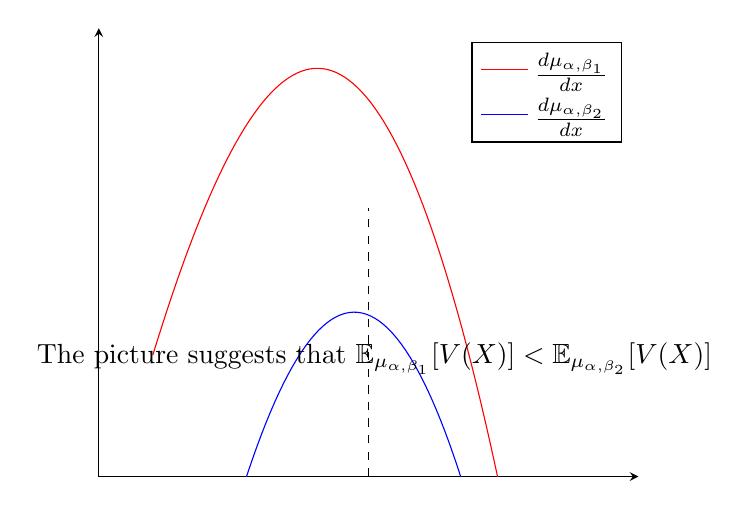
\begin{tikzpicture}
\begin{axis}[
    axis lines = left,
    xlabel = {},
    ylabel = {},
    ymin=0, ymax=2.5,
    xmin=0, xmax=5,
    ytick=\empty,
    xtick=\empty,
    legend pos=north east,
    legend cell align={left}
]
\addplot [
    domain=0.5:4.5, 
    samples=100, 
    color=red,
]
{-(x-2.5)^2 + 1.5*exp(-0.5*(x-2.5)) + 0.6};
\addlegendentry{$\frac{d\mu_{\alpha, \beta_1}}{dx}$}

\addplot [
    domain=0.5:4.5, 
    samples=100, 
    color=blue,
]
{-(x-2.5)^2 + 0.5*exp(-0.5*(x-2.5)) + 0.4};
\addlegendentry{$\frac{d\mu_{\alpha, \beta_2}}{dx}$}

\addplot[dashed, black] coordinates {(2.5,0) (2.5,1.5)};
\node at (axis cs:2.5,0) [anchor=north] {$\bar{x}$};

\end{axis}
\node at (3.5,1.5) {The picture suggests that $\mathbb{E}_{\mu_{\alpha, \beta_1}} [V(X)] < \mathbb{E}_{\mu_{\alpha, \beta_2}} [V(X)]$};
\end{tikzpicture}

\end{document}